\documentclass{article}
\usepackage[preprint]{neurips_2023}
\usepackage[T1]{fontenc}
\usepackage[utf8]{inputenc}
\usepackage{hyperref}
\usepackage{url}
\usepackage{booktabs}
\usepackage{amsfonts}
\usepackage{nicefrac}
\usepackage{microtype}
\usepackage{xcolor}
\usepackage{amsmath,amssymb,amsthm}
\usepackage{graphicx}
\usepackage{tabularx}
\usepackage{array}
\usepackage{enumitem}
\usepackage{multirow}
\usepackage{tikz}

\title{The Validity Mirage: Context Algebra for Endogenous Semantics under Memory Compression}
\author{Jack Chaudier Gaffney}

\newtheorem{theorem}{Theorem}
\newtheorem{proposition}{Proposition}
\newtheorem{definition}{Definition}
\newtheorem{remark}{Remark}

\begin{document}

\maketitle

\begin{abstract}
Modern long-context systems compress memory using truncation, eviction, or summarization, often evaluated by raw task validity. In endogenous-pivot settings, this is insufficient: feasibility depends on a turning point chosen by \texttt{argmax} over the selected sequence, so compression can alter semantics by changing pivot identity. We formalize a compositional context algebra over summaries $C=(w^\star,d_{\mathrm{total}},d_{\mathrm{pre}})$ and prove associativity of endogenous composition. Under committed semantics, we prove an absorbing left-ideal property and define a checkable no-absorption compression contract. Empirically, composition is exact and associative on tested cells (Exp51: 0 violations), absorbing closure holds (Exp56: 0/96 violations), and closure breaks appear only under compression (Exp57: 0.133 closure violation rate). Retention sweeps show the validity mirage: TP-conditioned raw validity remains near 1.0 while pivot preservation and fixed-pivot feasibility degrade sharply. A deterministic witness (Exp58) isolates the mechanism: naive compression is infeasible under committed semantics, while under multi-candidate semantics it appears feasible only via pivot substitution, with a 54.4\% score shortfall. The main conclusion is that compression safety must be defined relative to pivot consistency, not raw feasibility alone.
\end{abstract}

\section{Introduction}
Large language models and other long-sequence systems now depend on context management: truncation, cache eviction, retrieval, or summarization. Most evaluations ask whether the system still produces a valid output. That criterion is often too weak when semantics are endogenous.

Compression is often treated as structurally neutral: the past is assumed to be a concatenated string (a free monoid), and compression is treated as approximately semantics-preserving.

In endogenous settings, the interpretation of early context depends on a later turning point that is itself chosen from the selected sequence. Compression decisions that look locally safe can become globally unsafe once the eventual pivot is revealed. This is the mechanism behind many failures that appear as ``hallucination'' or ``drift'' but are structurally consistent under a changed internal hypothesis.

Our companion finite paper established a sharp sufficient-condition impossibility boundary (zero false positives in a validated 11{,}400-instance regime). Our companion streaming paper established irreversible commitment traps (54.9\% organic trap rate over 4{,}200 runs). This paper fills the compositional gap between those results: we define the algebra of context summaries under endogenous pivots and study when compression preserves or breaks that algebra.

\paragraph{Contributions.}
\begin{enumerate}[leftmargin=1.5em]
  \item We formalize a compact context monoid for endogenous pivots and provide full associativity and absorbing-ideal proofs under explicit semantics.
  \item We validate monoid exactness and ideal closure empirically (Exps 51 and 56), and identify compression as the unique tested closure-breaking operation (Exp57).
  \item We define semantic diagnostics (pivot preservation, fixed-pivot feasibility, semantic regret) and show why raw feasibility alone creates a validity mirage.
  \item We provide a deterministic witness (Exp58) that isolates semantic drift via pivot substitution and quantifies the resulting score loss.
\end{enumerate}

\section{Preliminaries and Semantics}
We consider extraction from temporally ordered event graphs with focal-actor turning points and prefix requirement $k$. For selected sequence $S$, endogenous turning point is
\[
\tau(S)=\arg\max_{v\in S,\,a(v)=a^*} w(v),
\]
with deterministic tie-breaking by $(w,-t,\mathrm{id})$.

We evaluate three solver semantics:
\begin{itemize}[leftmargin=1.3em]
  \item \textbf{Committed semantics:} pivot identity is fixed once chosen and cannot be replaced by later candidates.
  \item \textbf{Enumerative semantics:} solver evaluates top-$M$ pivot candidates and may return any feasible candidate.
  \item \textbf{Fixed-pivot semantics:} enumerative solver constrained to the full-sequence dominant pivot.
\end{itemize}

The TP-conditioned solver is a label-setting dynamic program over fixed-pivot subproblems, aligned with resource-constrained shortest-path formulations \citep{irnich2005shortest}.

\section{Context Algebra}
\subsection{Context element}
\begin{definition}[Context element]
A context summary is
\[
C=(w^\star,d_{\mathrm{total}},d_{\mathrm{pre}}),
\]
where $w^\star$ is the local pivot key, $d_{\mathrm{total}}$ is total development capacity in the block, and $d_{\mathrm{pre}}$ is development capacity before the local pivot.
\end{definition}

\subsection{Endogenous composition}
For adjacent blocks $A$ then $B$, define $C_{A\Vert B}=C_A\otimes_{\mathrm{endo}} C_B$:
\[
\begin{aligned}
w^\star &= \max(w^\star_A,w^\star_B),\\
d_{\mathrm{total}} &= d_{\mathrm{total},A}+d_{\mathrm{total},B},\\
d_{\mathrm{pre}} &=
\begin{cases}
 d_{\mathrm{pre},A}, & w^\star_A\ge w^\star_B,\\
 d_{\mathrm{total},A}+d_{\mathrm{pre},B}, & w^\star_B>w^\star_A.
\end{cases}
\end{aligned}
\]
The piecewise update is the critical term: if pivot shifts right, the entire left block becomes pre-pivot and contributes its full $d_{\mathrm{total}}$.

\paragraph{Committed vs endogenous operators.}
To make solver semantics explicit in the algebra (not only in prose), we separate two operators:
\begin{itemize}[leftmargin=1.3em]
  \item $\otimes_{\mathrm{endo}}$: pivot can be replaced by a higher suffix key (the definition above).
  \item $\otimes_{\mathrm{commit}}$: left committed pivot cannot be replaced.
\end{itemize}
For committed composition, use an extended element $\bar C=(w^\star,d_{\mathrm{total}},d_{\mathrm{pre}},\kappa)$ with commitment flag $\kappa\in\{0,1\}$:
\[
\bar C_A\otimes_{\mathrm{commit}}\bar C_B=
\begin{cases}
(w^\star_A,\ d_{\mathrm{total},A}+d_{\mathrm{total},B},\ d_{\mathrm{pre},A},\ 1), & \kappa_A=1,\\
\big((C_A\otimes_{\mathrm{endo}}C_B),\ \kappa_B\big), & \kappa_A=0.
\end{cases}
\]
Proposition~2 is stated over $\otimes_{\mathrm{commit}}$.

\subsection{Associativity}
\begin{proposition}[Associativity]
$\otimes_{\mathrm{endo}}$ is associative.
\end{proposition}
\begin{proof}
Let $A,B,C$ be three consecutive blocks, with strict total order on pivot keys from deterministic tie-breaking.

\textbf{Case 1: global pivot in $A$.} Then $w^\star_A\ge w^\star_B,w^\star_C$. For $(A\otimes B)\otimes C$, first composition yields $d_{\mathrm{pre},AB}=d_{\mathrm{pre},A}$ and $d_{\mathrm{total},AB}=d_{\mathrm{total},A}+d_{\mathrm{total},B}$. Composing with $C$ preserves pivot in $A$, so $d_{\mathrm{pre}}=d_{\mathrm{pre},A}$ and $d_{\mathrm{total}}=d_{\mathrm{total},A}+d_{\mathrm{total},B}+d_{\mathrm{total},C}$. For $A\otimes(B\otimes C)$, $A$ still dominates, giving the same pair $(d_{\mathrm{pre}},d_{\mathrm{total}})$.

\textbf{Case 2: global pivot in $B$.} Then $w^\star_B>w^\star_A,w^\star_C$. In $(A\otimes B)$, pivot shifts to $B$, so $d_{\mathrm{pre},AB}=d_{\mathrm{total},A}+d_{\mathrm{pre},B}$. Composing with $C$ preserves pivot in $B$, giving final $d_{\mathrm{pre}}=d_{\mathrm{total},A}+d_{\mathrm{pre},B}$. In $A\otimes(B\otimes C)$, $B\otimes C$ has pivot in $B$ and $d_{\mathrm{pre},BC}=d_{\mathrm{pre},B}$, so final $d_{\mathrm{pre}}=d_{\mathrm{total},A}+d_{\mathrm{pre},BC}=d_{\mathrm{total},A}+d_{\mathrm{pre},B}$.

\textbf{Case 3: global pivot in $C$.} Symmetrically, both parenthesizations yield
\[
d_{\mathrm{pre}}=d_{\mathrm{total},A}+d_{\mathrm{total},B}+d_{\mathrm{pre},C},
\]
with identical $d_{\mathrm{total}}$.

All cases agree; therefore $\otimes_{\mathrm{endo}}$ is associative.
\end{proof}

\begin{proposition}[Identity element]
Under the pivot-key order, $e=(-\infty,0,0)$ satisfies
\[
C\otimes_{\mathrm{endo}}e=e\otimes_{\mathrm{endo}}C=C.
\]
Hence $(\mathcal{C},\otimes_{\mathrm{endo}},e)$ is a monoid.
\end{proposition}
\begin{proof}
For $C=(w^\star,d_{\mathrm{total}},d_{\mathrm{pre}})$, composition with $e$ keeps pivot key $w^\star$, adds zero development mass, and leaves pre-pivot mass unchanged in both directions by the same case split as Definition 3.2.
\end{proof}

\paragraph{Systems implication.}
Because $\otimes$ is strictly associative, context reduction supports parallel tree reductions and therefore $O(\log n)$ reduction depth in recursive context trees.

\section{Absorbing Ideal and No-Absorption Contract}
Fix grammar parameter $k$ and define absorbing predicate $\bot$ by $d_{\mathrm{pre}}<k$ (applied to the $d_{\mathrm{pre}}$ component of either $C$ or $\bar C$).

\begin{proposition}[Absorbing left ideal under committed semantics]
If committed context $\bar A$ has $\kappa_A=1$ and $\bar A\in\bot$, then for any suffix context $\bar D$, $\bar A\otimes_{\mathrm{commit}}\bar D\in\bot$.
\end{proposition}
\begin{proof}
Under committed semantics, suffix events cannot replace the committed pivot. Hence
\[
d_{\mathrm{pre},\bar A\otimes_{\mathrm{commit}}\bar D}=d_{\mathrm{pre},\bar A}<k,
\]
so $\bar A\otimes_{\mathrm{commit}}\bar D\in\bot$ for all $\bar D$.
\end{proof}

\begin{remark}[Semantics qualifier]
Without commitment ($\otimes_{\mathrm{endo}}$), suffix pivot substitution can escape absorption: if $w^\star_D>w^\star_A$, then $d_{\mathrm{pre}}=d_{\mathrm{total},A}+d_{\mathrm{pre},D}$ may exceed $k$. Exp58 is an explicit witness of this distinction.
\end{remark}

\begin{definition}[No-absorption contract]
For grammar demand $k$, a compression map $\mu$ on block $B$ satisfies the no-absorption contract if
\[
d_{\mathrm{total}}(\mu(B)) \ge \min\!\big(d_{\mathrm{total}}(B),\,k\big).
\]
\end{definition}

This definition is checkable and operational: compression may remove redundant capacity, but it cannot reduce latent prefix-support below the threshold needed to survive a future pivot shift.

\section{Multi-Candidate Pivots and the Validity Mirage}
When solvers enumerate multiple pivot candidates ($M>1$), raw feasibility can remain high even after compression damages the dominant-pivot trajectory. The solver can recover feasibility by substituting a different pivot. We call this the \emph{validity mirage}.

We therefore evaluate three semantic diagnostics in addition to validity:
\begin{itemize}[leftmargin=1.3em]
  \item \textbf{Pivot preservation rate:} fraction of valid compressed solves that keep the full-sequence pivot.
  \item \textbf{Fixed-pivot feasibility:} validity when forcing compressed solve to the full-sequence pivot.
  \item \textbf{Semantic regret:} relative score shortfall against the full-sequence dominant-pivot trajectory.
\end{itemize}

\begin{figure}[t]
\centering
\includegraphics[width=\linewidth]{figures/validity_mirage_tp.pdf}
\caption{TP-conditioned sweep ($n=200$, $k=3$, $M=10$, 100 seeds). X-axis is compression rate $c=1-\mathrm{retention}$. Raw validity stays near 1.0 while pivot-preservation rates degrade as compression tightens.}
\label{fig:validity_mirage}
\end{figure}

\section{Experimental Protocol}
\paragraph{Artifacts and determinism.}
All experiments are deterministic and sourced from saved outputs in \path{experiments/output/}. We use context-algebra suite Exps 50--57, full-scale retention sweeps, and deterministic witness Exp58.

\paragraph{Diagnostic state.}
For taxonomy and closure diagnostics we use enriched state
\[
\mathcal{S}=(q,r,\Pi,t_{\min},t_{\max}),
\]
with grammar state $q$, counters $r$, pivot set $\Pi$, and temporal bounds. This directly enabled Exp50 predicate correction (failure-only Class-A accuracy from 0.000 to 1.000) and Exp57 mismatch diagnostics.

\paragraph{Compression strategies and semantics.}
We compare naive, bridge-preserving, and contract-guarded compression under TP-conditioned and greedy solvers. For TP-conditioned runs, each compressed solve is scored both in free mode and fixed-pivot mode.

\section{Results}
\subsection{Claim 1: The monoid is exact and the ideal is closed}
Table~\ref{tab:core_algebra} summarizes the core algebraic checks; all tested exactness and closure checks pass with zero violations.
\begin{table}[t]
\centering
\small
\begin{tabular}{lccc}
\toprule
Check & Cases/Checks & Violations & Rate \\
\midrule
Exp51 pairwise exact ($q/r$) & 240 & 0 & 0.000 \\
Exp51 pairwise exact (pivots) & 240 & 0 & 0.000 \\
Exp51 associativity & 80 & 0 & 0.000 \\
Exp56 absorbing-ideal closure & 96 & 0 & 0.000 \\
\bottomrule
\end{tabular}
\caption{Core algebraic checks: exactness and closure hold on tested cells.}
\label{tab:core_algebra}
\end{table}
With 0 observed violations in $n$ tested cells, the 95\% rule-of-three upper bound is approximately $3/n$ (e.g., $3/240\approx1.25\%$, $3/96\approx3.13\%$), so these results strongly constrain but do not prove impossibility outside the tested regime.

\subsection{Claim 2: Compression is the unique tested closure-breaking operation}
\begin{table}[t]
\centering
\small
\begin{tabular}{lcc}
\toprule
Operation & Closure violation rate & Absorbing escape rate \\
\midrule
Composition & 0.000 & 0.000 \\
Compression & 0.133 & 0.033 \\
Pivot update & 0.000 & 0.000 \\
Split-at-point & 0.000 & 0.000 \\
\bottomrule
\end{tabular}
\caption{Exp57 closure diagnostics by operation.}
\label{tab:exp57_closure}
\end{table}

Closure breakdown concentrates entirely in compression.

\subsection{Claim 3: Raw feasibility alone creates a validity mirage}
In full-scale Exp52/53, raw validity ties at 1.000 across naive/bridge/contract and segment-wise vs whole compression (gap 0.000). Semantic diagnostics reveal degradation despite this tie.

\begin{table}[t]
\centering
\small
\begin{tabular}{ccccc}
\toprule
Retention & Naive valid & Pivot preserve & Fixed-pivot valid & Semantic regret \\
\midrule
0.50 & 1.000 & 0.790 & 0.980 & 0.218 \\
0.30 & 1.000 & 0.590 & 0.920 & 0.663 \\
0.20 & 1.000 & 0.480 & 0.860 & 0.677 \\
0.10 & 0.990 & 0.354 & 0.750 & 0.358 \\
\bottomrule
\end{tabular}
\caption{Condensed TP-conditioned semantic sweep for naive compression (100 seeds, $M=10$). Raw validity stays high while pivot consistency degrades.}
\label{tab:tp_semantic_sweep}
\end{table}

Contract-guarded follows the same qualitative pattern; full per-strategy metrics are reported in Appendix~\ref{app:full_semantic_table}.
Semantic regret is non-monotone in the full sweep (Appendix~\ref{app:full_semantic_table}); at extreme compression, both full and compressed solves are often forced onto similarly degraded pivot candidates, reducing the measured gap.

\subsection{Claim 4: Solver semantics dominate compression strategy}
At retention 0.10 (same generator family, 100 seeds), TP-conditioned results are naive 0.990 vs contract 0.990, while greedy results are naive 0.000 vs contract 0.010. Dominant variance comes from solver semantics (committed/myopic vs enumerative), not compression heuristic alone.

\subsection{Claim 5: Exp58 isolates pivot substitution}
\begin{figure}[t]
\centering
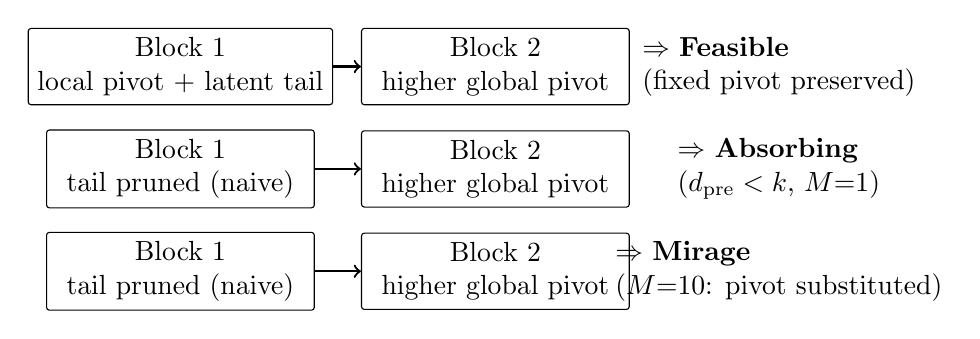
\begin{tikzpicture}[x=1cm,y=1cm]
  \tikzstyle{blk}=[draw,rectangle,rounded corners=1pt,minimum height=0.75cm,minimum width=3.4cm,align=center]
  \tikzstyle{arr}=[->,thick]

  % Row 1
  \node[blk] (b1a) at (0,0) {Block 1\\local pivot + latent tail};
  \node[blk] (b2a) at (4.0,0) {Block 2\\higher global pivot};
  \draw[arr] (b1a.east) -- (b2a.west);
  \node[align=left] at (7.6,0) {$\Rightarrow$ \textbf{Feasible}\\(fixed pivot preserved)};

  % Row 2
  \node[blk] (b1b) at (0,-1.3) {Block 1\\tail pruned (naive)};
  \node[blk] (b2b) at (4.0,-1.3) {Block 2\\higher global pivot};
  \draw[arr] (b1b.east) -- (b2b.west);
  \node[align=left] at (7.6,-1.3) {$\Rightarrow$ \textbf{Absorbing}\\($d_{\mathrm{pre}}<k$, $M{=}1$)};

  % Row 3
  \node[blk] (b1c) at (0,-2.6) {Block 1\\tail pruned (naive)};
  \node[blk] (b2c) at (4.0,-2.6) {Block 2\\higher global pivot};
  \draw[arr] (b1c.east) -- (b2c.west);
  \node[align=left] at (7.6,-2.6) {$\Rightarrow$ \textbf{Mirage}\\($M{=}10$: pivot substituted)};
\end{tikzpicture}
\caption{Exp58 mechanism diagram. Enumerative solvers can escape infeasibility by pivot substitution, yielding a validity mirage.}
\label{fig:exp58_diagram}
\end{figure}

\begin{table}[t]
\centering
\small
\begin{tabular}{lcccccc}
\toprule
Strategy & $M$ & Free valid & Free TP & Fixed-pivot valid & Pivot preserved & Score \\
\midrule
Naive & 1 & False & -- & False & False & -- \\
Contract-guarded & 1 & True & e41 & True & True & 47.084 \\
Naive & 10 & True & e45 & False & False & 21.467 \\
Contract-guarded & 10 & True & e41 & True & True & 47.084 \\
\bottomrule
\end{tabular}
\caption{Exp58 deterministic witness. Under $M=10$, naive is feasible only via pivot substitution (e45) and fails fixed-pivot feasibility.}
\label{tab:exp58}
\end{table}

Under committed semantics ($M=1$), Exp58 yields the witness triple: full feasible, naive infeasible, contract feasible. Under enumerative semantics ($M=10$), naive appears feasible only by changing pivot identity. Relative score shortfall versus the dominant-pivot trajectory is
\[
1-\frac{21.467}{47.084}=0.544.
\]

\clearpage
\section{Real-Incident External Validation}
We evaluate the same mechanism on 12 real incident causal graphs derived from NTSB aviation accident reports and the Knight Capital 2012 trading failure. For each incident we run compression at budgets $\{0.7,0.5,0.3\}$ with five seeds (60 trials per budget), then query \texttt{grok-4-1-fast-non-reasoning} for pivot selection under the same protocol used in synthetic runs.

\paragraph{Metric focus.}
We report pivot preservation, information shift, and silent mirage, where silent mirage means a degraded trial with a wrong pivot and no degraded-evidence flag.
In this run, model-side degraded-flag rate is 0 under both methods, so wrong-pivot cases are silent by default; the memory policy determines whether those wrong-pivot cases occur.
Silent-mirage rates are reported on degraded trials (method- and budget-specific denominators), while Wilson intervals use all 60 trials per budget as a fixed-denominator uncertainty bound.

\begin{table}[!ht]
\centering
\small
\begin{tabular}{lcccccc}
\toprule
Method & Budget & Retention & Info shift & Pivot preserve & Silent mirage (deg.) & Silent mirage CI (all 60) \\
\midrule
naive & 0.7 & 0.686859 & 40.0\% & 60.0\% & 12/51 (23.5\%) & 12/60, [11.83\%, 31.78\%] \\
contract & 0.7 & 0.686859 & 0.0\% & 100.0\% & 0/4 (0.0\%) & 0/60, [0.00\%, 6.02\%] \\
naive & 0.5 & 0.478276 & 55.0\% & 45.0\% & 11/56 (19.6\%) & 11/60, [10.56\%, 29.92\%] \\
contract & 0.5 & 0.487536 & 0.0\% & 100.0\% & 0/8 (0.0\%) & 0/60, [0.00\%, 6.02\%] \\
naive & 0.3 & 0.313141 & 76.7\% & 23.3\% & 13/57 (22.8\%) & 13/60, [13.12\%, 33.62\%] \\
contract & 0.3 & 0.450570 & 0.0\% & 100.0\% & 0/10 (0.0\%) & 0/60, [0.00\%, 6.02\%] \\
\bottomrule
\end{tabular}
\caption{Real-incident external validation with xAI non-reasoning backend. Primary matched-retention comparison is budget 0.7 vs 0.7 (identical achieved retention). ``Silent mirage (deg.)'' uses degraded-trial denominators; the CI column uses all 60 trials per cell.}
\label{tab:real_incident_validation}
\end{table}

Overall naive silent mirage is 36/164 = 21.95\% (Wilson 95\% CI [16.30\%, 28.89\%]) across degraded rows; contract remains at 0\% in every budget cell in this run.

\paragraph{Mechanism check at matched retention.}
At budget 0.7, achieved retention is identical between methods (0.686859 vs 0.686859), yet naive shows 23.5\% degraded silent mirage while contract remains at 0\%. This isolates prerequisite preservation as the mechanism, not raw retained volume.
The same pattern appears in near-match comparison (naive 0.5 retention 0.478 vs contract 0.3 retention 0.451): naive still exhibits silent mirage while contract remains at 0.
Contract therefore outperforms naive even at lower achieved retention (0.451 $<$ 0.478).
Mean prerequisite support ratio is substantially higher for contract (0.967--0.987 across budgets) than naive (0.319--0.668), matching the contract's design objective.

\section{Additional External Validation}
\subsection{Multi-model blackbox validation}
We evaluated five architectures (Llama 3.1 8B, Mistral 7B v0.3, Gemma 2 9B, Phi-3 Medium 14B, Qwen 2.5 14B), all in bf16 on H100 with greedy decoding ($\texttt{do\_sample=False}$), on the same 12-task MirageBench set and compression levels $\{0.4,0.5,0.6\}$ used in prior Qwen blackbox runs. Metric definitions and pivot extraction are identical to the main benchmark stack.

\begin{table}[t]
\centering
\small
\begin{tabular}{lccccc}
\toprule
Model & Raw validity & Pivot preserve & Fixed-pivot feasible & Semantic regret & Valid but switched \\
\midrule
Llama 3.1 8B & 0.962 & 0.417 & 0.222 & 0.260 & 0.583 \\
Mistral 7B v0.3 & 0.926 & 0.611 & 0.222 & 0.238 & 0.389 \\
Gemma 2 9B & 0.885 & 0.667 & 0.083 & 0.306 & 0.333 \\
Phi-3 Medium 14B & 0.835 & 0.444 & 0.222 & 0.208 & 0.417 \\
Qwen 2.5 14B & 0.954 & 0.722 & 0.167 & 0.307 & 0.278 \\
\bottomrule
\end{tabular}
\caption{Per-model blackbox results on MirageBench (180 rows total). ``Valid but switched'' is $\mathbf{1}[\text{raw\_validity}>0.5\ \wedge\ \text{pivot\_preserved}=0]$.}
\label{tab:blackbox_multimodel}
\end{table}

\begin{table}[t]
\centering
\small
\begin{tabular}{lccccc}
\toprule
Category & Raw validity & Pivot preserve & Fixed-pivot feasible & Semantic regret & Valid but switched \\
\midrule
Incident & 0.931 & 0.800 & 0.033 & 0.230 & 0.183 \\
Investment & 0.896 & 0.200 & 0.517 & 0.296 & 0.800 \\
Narrative & 0.910 & 0.717 & 0.000 & 0.265 & 0.217 \\
\bottomrule
\end{tabular}
\caption{Category-pooled blackbox metrics across all five models.}
\label{tab:blackbox_category}
\end{table}

The validity mirage pattern is consistent across all five models from four vendors: responses remain high-validity while pivot preservation drops. Investment is the fragile basin (20\% pivot preservation versus 80\% for incident), matching the qualitative regime split predicted by Exp57/Exp58.

\subsection{KV-cache eviction (representation-level mirage)}
To test representation-level degradation, we ran Llama 3.1 8B (bf16) with full prompt prefill, then applied middle-out KV eviction: keep a fixed anchor prefix (first 256 positions) plus a suffix window, evict the middle, at retention $\{1.0,0.7,0.5,0.3,0.1\}$. This approximates production cache management with attention-sink preservation \citep{xiao2023streamingllm} and includes retention 1.0 as control.

\begin{table}[t]
\centering
\small
\begin{tabular}{lccccc}
\toprule
Retention & Header compliance & Pivot preserve (all) & Pivot preserve ($\mid$ header) & Raw validity & Semantic regret \\
\midrule
1.0 & 0.917 & 1.000 & 1.000 & 0.962 & 0.000 \\
0.7 & 0.500 & 0.583 & 0.833 & 0.703 & 0.320 \\
0.5 & 0.833 & 0.500 & 0.600 & 0.508 & 0.375 \\
0.3 & 0.417 & 0.167 & 0.200 & 0.629 & 0.375 \\
0.1 & 0.667 & 0.083 & 0.000 & 0.680 & 0.330 \\
\bottomrule
\end{tabular}
\caption{KV-eviction validation (60 rows total). Header compliance is $\mathbf{1}[\texttt{PIVOT\_ID=} \text{ emitted}]$.}
\label{tab:kv_eviction}
\end{table}

In this experiment, fixed-pivot feasibility is 1.0 at every retention level because all prerequisite information remains in the input text. Yet pivot preservation degrades sharply with retention, and on protocol-compliant outputs falls from 1.000 (retention 1.0) to 0.000 (retention 0.1). This is representation-level validity mirage: evidence is present in input but inaccessible after cache eviction.

The KV setting also separates two degradation modes: (a) protocol collapse (model stops emitting the required \texttt{PIVOT\_ID=} structure and recites raw events), and (b) silent pivot substitution (header-compliant but wrong pivot). We treat (b) as the mirage proper and (a) as an orthogonal protocol-level degradation.

\section{Related Work}
Our framing is algebraic: context summaries are composed under an endogenous operator with explicit invariants, analogous in spirit to how relational algebra formalizes data operations \citep{codd1970relational}. On the combinatorial side, endogenous pivot selection with prefix constraints falls outside hereditary/exchange structures that support classical greedy guarantees \citep{korte1981mathematical,bjorner1992greedoids}.

Long-context modeling work typically emphasizes scalable mechanisms without formal compression-safety guarantees. This includes sparse/sliding attention (Longformer \citep{beltagy2020longformer}), positional extrapolation methods (RoFormer \citep{su2021roformer}; positional interpolation \citep{chen2023position}), retrieval-augmented systems (REALM \citep{guu2020realm}, RAG \citep{lewis2020rag}), state-space sequence models (Mamba \citep{gu2023mamba}), KV-cache policies (H$_2$O \citep{zhang2023h2o}), and persistent memory architectures (MemoryBank \citep{zhong2023memorybank}). Our contribution is complementary: an algebraic safety layer for pivot-consistent feasibility under compression.

\section{Discussion and Limitations}
\paragraph{What is established.}
Composition behaves as a stable algebraic object on tested cells; absorbing closure is robust under committed semantics; compression is the unique tested closure-breaking operation.

\paragraph{Interpretation.}
The key lesson is not ``contract always improves validity.'' The key lesson is that validity can hide semantic drift under multi-candidate pivot substitution. Safety criteria must include pivot consistency.

\paragraph{Implications for long-context systems.}
An LLM can produce coherent outputs after aggressive compression while internally switching to an alternate hypothesis. This suggests one plausible mechanism for semantic drift and some forms of hallucination: not arbitrary fabrication ex nihilo, but coherent continuation of a degraded hypothesis after critical latent constraints were removed.

\paragraph{Limitations.}
Exp58 is a deterministic witness, not a distributional guarantee. Real-incident validation is still small-scale (12 incidents, single-model backend), while most sweeps remain synthetic. The multi-model blackbox sweep remains a 12-task benchmark, and KV eviction is currently single-model with one eviction strategy (middle-out anchor + suffix). At aggressive retention (0.3/0.1), protocol collapse is common, so the cleanest mirage signal is at moderate retention (0.5--0.7). A full symbolic characterization of compression-safe contracts beyond the threshold form above remains open.

\section{Conclusion}
Context algebra separates structural composition from policy effects in endogenous-pivot sequential systems. The monoid and absorbing ideal are stable under composition; compression marks the main boundary where invariants fail. Semantic instrumentation reveals a validity mirage in strong solvers, and Exp58 isolates the pivot-substitution mechanism. More broadly, extending the committed-pivot monoid to a multi-candidate algebra that composes over time while selecting across pivot hypotheses suggests a set-valued lift; we conjecture this forms a context semiring under persistent pivot uncertainty, and a natural direction for hierarchical context management in systems with endogenous semantics.
Real-incident validation on NTSB-derived accident graphs confirms silent pivot substitution at roughly 22\% under naive compression with a frontier LLM, eliminated by the no-absorption contract in this run.

\section*{Reproducibility Artifacts}
Primary artifacts used in this manuscript:
\begin{itemize}[leftmargin=1.3em]
  \item \path{context_algebra_suite.json}
  \item \path{context_algebra_suite_refined2.json}
  \item \path{context_algebra_exp52_53_n200_m510.json}
  \item \path{context_retention_sweep_tp_semantics_m10.json}
  \item \path{context_retention_sweep_greedy_semantics_m10.json}
  \item \path{exp58_pivot_shift_witness_semantics.json}
\end{itemize}

\appendix
\section{Full TP Semantic Sweep Table}
\label{app:full_semantic_table}
\begin{table}[h]
\centering
\footnotesize
\begin{tabular}{cccccccc}
\toprule
$r$ & N val & C val & N piv & C piv & N fix & C fix & Gap rej \\
\midrule
0.50 & 1.000 & 1.000 & 0.790 & 0.770 & 0.980 & 0.990 & 112.23 \\
0.45 & 1.000 & 1.000 & 0.730 & 0.700 & 0.970 & 0.980 & 154.16 \\
0.40 & 1.000 & 1.000 & 0.700 & 0.670 & 0.970 & 0.960 & 196.30 \\
0.35 & 1.000 & 1.000 & 0.630 & 0.570 & 0.960 & 0.940 & 238.63 \\
0.30 & 1.000 & 1.000 & 0.590 & 0.580 & 0.920 & 0.930 & 281.21 \\
0.25 & 1.000 & 1.000 & 0.500 & 0.450 & 0.890 & 0.910 & 324.18 \\
0.20 & 1.000 & 0.990 & 0.480 & 0.404 & 0.860 & 0.890 & 367.77 \\
0.15 & 0.990 & 0.990 & 0.394 & 0.333 & 0.850 & 0.870 & 412.66 \\
0.10 & 0.990 & 0.990 & 0.354 & 0.354 & 0.750 & 0.780 & 459.45 \\
\bottomrule
\end{tabular}
\caption{Full TP-conditioned semantic sweep (all retention points). Abbreviations: N = naive, C = contract-guarded, piv = pivot-preservation rate, fix = fixed-pivot feasibility, Gap rej = mean rejected gap-guard drops.}
\end{table}

\section{Supporting Results: Deferred Composition and Recursive Depth}
These results are retained as supporting evidence, not central claims.

\paragraph{Exp54 (deferred composition).}
Suite diagnostics show nonzero patience dominates $f=0$ by the configured dominance check. Aggregate values: valid rate at $f=0.00$ is 1.000 (mean pivot shifts 0.639), while $f=0.25$ and $f=0.50$ remain 1.000 with reduced shift rates (0.333 and 0.111).

\paragraph{Exp55 (recursive depth).}
Refined target checks report all defined cells at or above 90\% validity retention versus flat baseline (5/5 defined cells). One cell ($n=500$, block size 50) has both recursive and flat validity equal to 0, yielding undefined retention ratio (n/a).

\bibliographystyle{plainnat}
\bibliography{references}

\end{document}
